\documentclass[12pt]{article}
\usepackage[utf8]{inputenc}
\usepackage[T1]{fontenc}
\usepackage[english]{babel}
\usepackage[a4paper,margin=2.5cm]{geometry}
\usepackage{amsmath}
\usepackage{graphicx}
\usepackage{tikz}
\usepackage{listings}
\usepackage{xcolor}
\usepackage{booktabs}
\usetikzlibrary{arrows.meta,positioning}

\definecolor{codegray}{rgb}{0.95,0.95,0.95}
\lstset{
    basicstyle=\ttfamily\small,
    backgroundcolor=\color{codegray},
    frame=single,
    breaklines=true,
    columns=fullflexible
}

\title{Implementation and Verification of the Full UART System}
\author{}
\date{}

\begin{document}

\maketitle

\section{Objective}

The folder \texttt{VERIFICATION/uart-full/} extends the previous
transmitter-only work into a complete UART subsystem. The final result is a
small but complete 8N1 UART solution composed of:

\begin{itemize}
    \item a transmitter in \texttt{src/uart\_tx.v},
    \item a receiver in \texttt{src/uart\_rx.v},
    \item and a top-level wrapper in \texttt{src/top.v}.
\end{itemize}

The goal of this report is to explain both the implementation and the
verification strategy of that full system. A special point in this assignment is
the receive path: the external UART input \texttt{rx} does not arrive aligned to
the local system clock, so the receiver must handle a clock-domain crossing
issue before it can decode serial data safely.

\section{Final Files}

The final \texttt{uart-full} folder contains:

\begin{lstlisting}[language=bash]
src/uart_tx.v
src/uart_rx.v
src/top.v
tb/tb_uart_tx.v
tb/tb_uart_rx.v
tb/tb_top.v
\end{lstlisting}

The three source files implement the system, and the three testbenches verify it
at different levels:

\begin{itemize}
    \item \texttt{tb\_uart\_tx.v}: dedicated verification of the transmitter,
    \item \texttt{tb\_uart\_rx.v}: dedicated verification of the receiver,
    \item \texttt{tb\_top.v}: integration verification of the full UART system.
\end{itemize}

\section{UART System Overview}

The implemented design is a basic UART with the classic 8N1 frame format:

\begin{itemize}
    \item 1 start bit with value \texttt{0},
    \item 8 data bits,
    \item 1 stop bit with value \texttt{1}.
\end{itemize}

The transmitter sends data LSB first, and the receiver reconstructs data in that
same order.

\subsection*{Top-Level Interface}

\begin{lstlisting}[language=Verilog]
module top #(
    parameter CLK_FREQ  = 27_000_000,
    parameter BAUD_RATE = 115200
)(
    input  wire       clk,
    input  wire       rst_n,
    input  wire       tx_en,
    input  wire [7:0] tx_data,
    input  wire       rx,
    output wire       tx,
    output wire       tx_busy,
    output wire [7:0] rx_data,
    output wire       rx_done,
    output wire       rx_busy,
    output wire       rx_frame_error
);
\end{lstlisting}

Two important architectural decisions are visible here:

\begin{itemize}
    \item \texttt{rst\_n} is an active-low reset shared by the TX and RX blocks.
    \item \texttt{tx} and \texttt{rx} are independent serial lines, so the system
    is full duplex.
\end{itemize}

That means the design can transmit and receive at the same time.

\section{Timing Parameters}

The TX and RX modules both use the same timing definition:

\begin{lstlisting}[language=Verilog]
localparam integer CLOCKS_PER_BIT = CLK_FREQ / BAUD_RATE;
\end{lstlisting}

With the default values:

\begin{itemize}
    \item \texttt{CLK\_FREQ = 27\_000\_000}
    \item \texttt{BAUD\_RATE = 115200}
\end{itemize}

the design obtains:

\[
\texttt{CLOCKS\_PER\_BIT} =
\left\lfloor \frac{27\,000\,000}{115200} \right\rfloor = 234
\]

As in the transmitter-only version, this is integer division, so the generated
bit period is an approximation of the requested baud rate.

In the full version, both TX and RX also compute an internal counter width from
\texttt{CLOCKS\_PER\_BIT}. This avoids a fixed-size counter and makes the design
more robust if the parameters are changed later.

\section{Architecture of the Full UART System}

\begin{figure}[h!]
\centering
\resizebox{\textwidth}{!}{
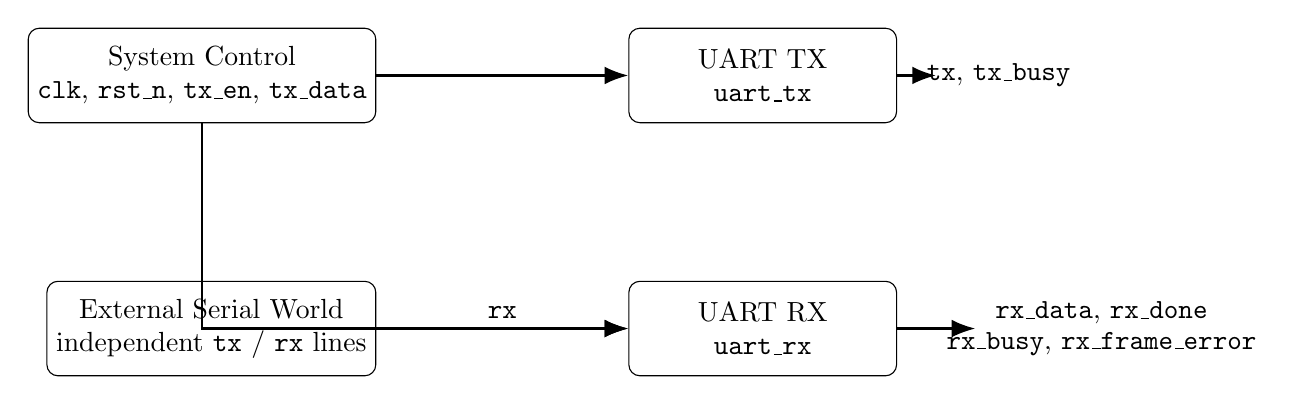
\begin{tikzpicture}[
    box/.style={draw, rounded corners, minimum width=3.4cm, minimum height=1.2cm, align=center},
    arrow/.style={-{Latex[length=3mm]}, thick}
]
    \node[box] (ctrl) {System Control\\\texttt{clk}, \texttt{rst\_n}, \texttt{tx\_en}, \texttt{tx\_data}};
    \node[box, right=3.2cm of ctrl] (tx) {UART TX\\\texttt{uart\_tx}};
    \node[box, below=2.0cm of tx] (rx) {UART RX\\\texttt{uart\_rx}};
    \node[box, left=3.2cm of rx] (line) {External Serial World\\independent \texttt{tx} / \texttt{rx} lines};

    \draw[arrow] (ctrl) -- (tx);
    \draw[arrow] (ctrl) |- (rx);
    \draw[arrow] (tx) -- node[right] {\texttt{tx}, \texttt{tx\_busy}} ++(2.2,0);
    \draw[arrow] (line) -- node[above] {\texttt{rx}} (rx);
    \draw[arrow] (rx) -- node[right] {\shortstack{\texttt{rx\_data}, \texttt{rx\_done} \\
    \texttt{rx\_busy}, \texttt{rx\_frame\_error}}} ++(2.7,0);
\end{tikzpicture}
}
\caption{High-level structure of the full UART system.}
\end{figure}

The top-level module itself is intentionally simple. It does not add another
state machine. Instead, it instantiates one transmitter and one receiver in
parallel, both driven by the same \texttt{clk} and the same active-low reset.

Because the data directions are independent, the design is naturally
full duplex:

\begin{itemize}
    \item the TX block can shift out a frame on \texttt{tx},
    \item while the RX block simultaneously samples a different frame on
    \texttt{rx}.
\end{itemize}

\section{Transmitter Role in the Full System}

The transmitter keeps the same 8N1 behavior already verified in the previous
UART work:

\begin{itemize}
    \item it waits in \texttt{s\_IDLE},
    \item it captures \texttt{tx\_data} when \texttt{tx\_en} is accepted,
    \item it transmits start, 8 data bits, and stop,
    \item and it keeps \texttt{tx\_busy} asserted during the active frame.
\end{itemize}

In the \texttt{uart-full} version, the main implementation improvement is the
counter width calculation. Instead of assuming a fixed 16-bit counter, the module
computes a width from \texttt{CLOCKS\_PER\_BIT}. That makes the timing logic
cleaner and avoids width-mismatch issues when linting or changing parameters.

\section{Receive Clock-Domain Issue}

The receive path is the most delicate part of the full system.

\subsection*{Why There Is a Clock-Domain Problem}

The external \texttt{rx} signal comes from another device or another timing
source. Even if both systems use the same nominal baud rate, the edge on
\texttt{rx} does not arrive synchronized to the local \texttt{clk}. Therefore:

\begin{itemize}
    \item the line can change very close to a clock edge,
    \item a flip-flop that samples it can enter metastability,
    \item and direct single-stage sampling can produce unreliable bit detection.
\end{itemize}

This is a classic clock-domain crossing issue: the UART line is effectively
asynchronous with respect to the receiver clock.

\subsection*{How the Design Solves It}

The implemented receiver uses a two-stage synchronizer:

\begin{lstlisting}[language=Verilog]
reg rx_meta;
reg rx_sync;
reg rx_sync_prev;

rx_meta      <= rx;
rx_sync      <= rx_meta;
rx_sync_prev <= rx_sync;
\end{lstlisting}

This solves two practical problems:

\begin{itemize}
    \item \texttt{rx\_meta} and \texttt{rx\_sync} reduce the metastability risk by
    resynchronizing the input to the local clock domain,
    \item \texttt{rx\_sync\_prev} makes it possible to detect the synchronized
    falling edge of the start bit.
\end{itemize}

The start condition is recognized with:

\begin{lstlisting}[language=Verilog]
if (rx_sync_prev && !rx_sync)
\end{lstlisting}

That edge only causes a transition into the receive sequence after the signal has
already been brought into the local clock domain.

\subsection*{Why Mid-Bit Sampling Is Used}

After detecting a possible start edge, the receiver does not immediately trust
the frame. It first waits approximately half a bit time:

\begin{lstlisting}[language=Verilog]
localparam integer START_TICKS = (CLOCKS_PER_BIT > 1) ?
                                 (CLOCKS_PER_BIT / 2) : 1;
\end{lstlisting}

Then it checks whether the line is still low. This has two benefits:

\begin{itemize}
    \item it confirms that the start bit is real and not just a short glitch,
    \item it places the sampling point near the middle of the start bit.
\end{itemize}

Once the start bit is confirmed, the receiver samples each data bit once per bit
period. In this implementation, that means one sample every
\texttt{CLOCKS\_PER\_BIT} clock cycles. This places the sampling point near the
center of each bit period and makes the UART receiver tolerant to small phase
differences between the transmitting and receiving clocks.

\section{Receiver State Machine}

The receive state machine has four states:

\begin{itemize}
    \item \texttt{s\_IDLE}
    \item \texttt{s\_START}
    \item \texttt{s\_DATA}
    \item \texttt{s\_STOP}
\end{itemize}

\subsection*{\texttt{s\_IDLE}}

In \texttt{s\_IDLE}, the receiver waits for the synchronized falling edge of the
start bit. During this state:

\begin{itemize}
    \item \texttt{rx\_busy = 0},
    \item the counters are cleared,
    \item and the line is continuously observed for a new frame.
\end{itemize}

\subsection*{\texttt{s\_START}}

In \texttt{s\_START}, the receiver waits half a bit time and checks that the line
is still low. If it is no longer low, the event is treated as a false start and
the FSM returns to \texttt{s\_IDLE}.

\subsection*{\texttt{s\_DATA}}

In \texttt{s\_DATA}, the receiver waits one full bit time between samples and
stores the synchronized line value into:

\begin{lstlisting}[language=Verilog]
rx_shift[bit_index] <= rx_sync;
\end{lstlisting}

Because \texttt{bit\_index} starts at 0, the receiver reconstructs the byte in
LSB-first order, matching the transmitter.

\subsection*{\texttt{s\_STOP}}

In \texttt{s\_STOP}, the receiver samples the stop bit after one bit time:

\begin{itemize}
    \item if the line is high, the frame is accepted, \texttt{rx\_data} is updated,
    and \texttt{rx\_done} pulses for one clock,
    \item if the line is low, a framing error is reported with a one-cycle
    \texttt{rx\_frame\_error} pulse.
\end{itemize}

\section{Top Module Behavior}

The file \texttt{src/top.v} simply connects the two previously described blocks:

\begin{itemize}
    \item \texttt{uart\_tx} handles outgoing traffic,
    \item \texttt{uart\_rx} handles incoming traffic,
    \item both share \texttt{clk} and \texttt{rst\_n},
    \item and both operate independently.
\end{itemize}

This independence is what makes the module full duplex. The top-level block does
not force loopback internally. Instead, it exposes one TX line and one RX line.
Loopback is only created inside the integration testbench when that specific
verification scenario is desired.

\section{Why the Testbenches Use Reduced Parameters}

The implementation is parameterized for a realistic default clock and baud rate,
but the testbenches use smaller values:

\begin{lstlisting}[language=Verilog]
localparam integer CLK_FREQ       = 100_000;
localparam integer BAUD_RATE      = 1_000;
localparam integer CLOCKS_PER_BIT = CLK_FREQ / BAUD_RATE;
\end{lstlisting}

Therefore:

\[
\texttt{CLOCKS\_PER\_BIT} = 100
\]

This keeps the verification cycle-accurate while reducing simulation time. The
clock is still two orders of magnitude faster than the baud rate, so the timing
relationship remains representative.

\section{Verification Strategy}

The full solution is verified at three levels.

\subsection*{1. Dedicated TX Verification}

\texttt{tb/tb\_uart\_tx.v} keeps the self-checking strategy from the previous
work. It verifies:

\begin{itemize}
    \item reset behavior,
    \item nominal frame timing,
    \item LSB-first ordering,
    \item data capture semantics,
    \item busy overlap behavior,
    \item held-high reacceptance semantics,
    \item and back-to-back transfers.
\end{itemize}

Its checking style is cycle-based: it verifies entire bit windows and keeps
\texttt{tx\_busy} under observation throughout the frame.

\subsection*{2. Dedicated RX Verification}

\texttt{tb/tb\_uart\_rx.v} focuses on the receive path and, importantly, drives
the serial line asynchronously with respect to the local clock. That is why the
stimulus tasks use small start offsets such as 1, 2, 3, 4, 5, 6, and 7 ns rather
than always changing \texttt{rx} exactly on a clock edge.

This is important because it exercises the exact problem the receiver is supposed
to solve: a serial input that is not phase-aligned to \texttt{clk}.

The RX testbench verifies:

\begin{itemize}
    \item reset behavior,
    \item a nominal asynchronously timed frame,
    \item multiple data patterns,
    \item rejection of a false start,
    \item framing error detection,
    \item and back-to-back legal receptions.
\end{itemize}

\subsection*{3. Top-Level Integration Verification}

\texttt{tb/tb\_top.v} verifies the combined system and proves that the wrapper is
really full duplex.

It includes three different integration scenarios:

\begin{itemize}
    \item an external receive path using \texttt{ext\_rx},
    \item a simultaneous independent TX and RX case,
    \item and a loopback mode used only inside the testbench.
\end{itemize}

The full-duplex case is the most important integration check. In that test:

\begin{itemize}
    \item the transmitter sends one byte,
    \item the receiver samples another byte on an independent RX line,
    \item both operations overlap in time,
    \item and the testbench confirms that TX and RX can remain active
    simultaneously.
\end{itemize}

\section{Summary of Tested Cases}

\subsection*{TX Testbench Cases}

\begin{center}
\begin{tabular}{@{}ll@{}}
\toprule
\textbf{Case} & \textbf{Purpose} \\
\midrule
1 & Reset behavior \\
2 & Single nominal transmission \\
3 & Pattern sensitivity and LSB-first ordering \\
4 & Data capture vs later \texttt{tx\_data} changes \\
5 & Short overlapping request while busy is ignored \\
6 & Held-high \texttt{tx\_en} causes legal immediate reacceptance \\
7 & Back-to-back legal transmissions \\
\bottomrule
\end{tabular}
\end{center}

\subsection*{RX Testbench Cases}

\begin{center}
\begin{tabular}{@{}ll@{}}
\toprule
\textbf{Case} & \textbf{Purpose} \\
\midrule
1 & Reset behavior \\
2 & Single asynchronous nominal reception \\
3 & Pattern sensitivity and LSB-first decoding \\
4 & False start is rejected \\
5 & Bad stop bit raises framing error \\
6 & Back-to-back legal receptions \\
\bottomrule
\end{tabular}
\end{center}

\subsection*{Top Testbench Cases}

\begin{center}
\begin{tabular}{@{}ll@{}}
\toprule
\textbf{Case} & \textbf{Purpose} \\
\midrule
1 & Active-low reset behavior \\
2 & External receive path through top \\
3 & Simultaneous independent TX and RX \\
4 & Single TX to RX loopback \\
5 & Back-to-back loopback transfers \\
\bottomrule
\end{tabular}
\end{center}

\section{Validation Command}

The final validation was executed from the \texttt{VERIFICATION/} directory with:

\begin{lstlisting}[language=bash]
./builder-verification.sh -r uart-full -x -w
\end{lstlisting}

That flow:

\begin{itemize}
    \item compiled all three testbenches,
    \item executed all simulations,
    \item generated the waveform files,
    \item and launched GTKWave in the background.
\end{itemize}

The generated waveforms were:

\begin{itemize}
    \item \texttt{uart-full/build/tb\_top.vcd}
    \item \texttt{uart-full/build/tb\_uart\_rx.vcd}
    \item \texttt{uart-full/build/tb\_uart\_tx.vcd}
\end{itemize}

\section{Final Execution Results}

The final simulation log reported:

\begin{center}
\begin{tabular}{@{}lccc@{}}
\toprule
\textbf{Testbench} & \textbf{Cases} & \textbf{Checks} & \textbf{Failures} \\
\midrule
\texttt{tb\_top}     & 5 & 100   & 0 \\
\texttt{tb\_uart\_rx} & 6 & 121   & 0 \\
\texttt{tb\_uart\_tx} & 7 & 24106 & 0 \\
\bottomrule
\end{tabular}
\end{center}

In total, the complete verification campaign executed:

\begin{itemize}
    \item 18 highlighted cases,
    \item 24327 individual checks,
    \item and 0 failures.
\end{itemize}

This means:

\begin{itemize}
    \item the transmitter behavior is correct,
    \item the receiver correctly handles asynchronous sampling, false starts, and
    stop-bit errors,
    \item and the top-level wrapper correctly supports active-low reset and
    full-duplex operation.
\end{itemize}

\section{Conclusion}

The final \texttt{uart-full} implementation is no longer only a UART transmitter;
it is a complete UART subsystem with:

\begin{itemize}
    \item a parameterized TX path,
    \item a synchronized RX path,
    \item and a simple full-duplex top-level integration.
\end{itemize}

The most important design addition is the receiver clock-domain handling. The
external \texttt{rx} line is asynchronous to the local clock, so the design first
synchronizes it and then samples near the centers of the serial bits. That makes
the receiver much more realistic and robust than a direct raw-input sampler.

The verification strategy matches that design intent. Instead of using only a
single integration test, the work verifies:

\begin{itemize}
    \item the transmitter in isolation,
    \item the receiver in isolation,
    \item and the composed top-level system.
\end{itemize}

Because all three self-checking testbenches passed with zero failures, the final
result gives confidence not only in nominal UART transfers, but also in reset
behavior, asynchronous receive timing, framing-error reporting, back-to-back
operation, and true simultaneous transmit/receive behavior.

\end{document}
